\makeatletter
\let\blx@rerun@biber\relax
\makeatother

\documentclass{article}

\usepackage{arxiv}

\usepackage{lipsum}

\usepackage[utf8]{inputenc} % allow utf-8 input
\usepackage[T1]{fontenc}    % use 8-bit T1 fonts
\usepackage{hyperref}       % hyperlinks
\usepackage{url}            % simple URL typesetting
\usepackage{booktabs}       % professional-quality tables
\usepackage{amsfonts}       % blackboard math symbols
\usepackage{nicefrac}       % compact symbols for 1/2, etc.
\usepackage{microtype}      % microtypography
\usepackage{graphicx}
\graphicspath{ {./images/} }

\usepackage[natbib=true]{biblatex}
\usepackage{amsmath}
\usepackage{amssymb}
\usepackage{amsthm}
\usepackage{stmaryrd}
\usepackage{algorithmic,algorithm}
\usepackage{graphicx}
\usepackage{caption}
\usepackage{subcaption}
\usepackage{tikz}
\usetikzlibrary{positioning}
\usepackage{comment}
\usepackage{todonotes}
\usepackage{newclude}


\newcommand{\cX}{\mathcal{X}}
\newcommand{\cL}{\mathcal{L}}
\newcommand{\cY}{\mathcal{Y}}

\newcommand{\bX}{\mathbf{X}}
\newcommand{\bY}{\mathbf{Y}}

\newtheorem{definition}{Definition}
\newtheorem{remark}{Remark}
\newtheorem{proposition}{Proposition}
\newtheorem{corollary}{Corollary}

\title{Generative Object Detection Models for Mobile Robotics Applications}


\author{
 van Genuchten, H.J.M, \\
 ID: 1297333\\
 Artificial Intelligence and Data Engineering Lab\\
Eindhoven University of Technology\\
  \texttt{h.j.m.v.genuchten@student.tue.nl} \\
  \and
    \textbf{Dr. Tomczak, J. M.} \\
    Artificial Intelligence and Data Engineering Lab \\
    Eindhoven University of Technology \\
    \texttt{j.m.tomczak@tue.nl} \\
    \and
    \textbf{Keulen, B.} \\
    Avular \\
    \texttt{b.keulen@avular.com}

}

\addbibresource{references.bib}

\begin{document}
%%------------------------------------------------------------------------------
\include*{chapters/abstract}

%%------------------------------------------------------------------------------
\include*{chapters/introduction}


%%------------------------------------------------------------------------------
\section{Research approach}
\label{sec:approach}
%%------------------------------------------------------------------------------
\subsection{Overall methodology and decomposition}

% This subsection should explain the methodology that will be used during the project. You do not need to enter into details of the methods, tools, techniques (this will appear in the next subsection) but to explain the high-level methodology, including potentially how you will break the problem into smaller parts in order to attack it properly.

The project consist of 2 (+ 1 possible extension) parts, the first is the reproduction of LDMSeg \cite{vangansbeke2024ldmseg}. The second part will be the extension of that work by adding UQ to it. Possibly adapting ideas from \citep{gasperini2023segmenting} to the generative approach of LDMSeg. Finally, if time permits an extension to temporal data will be made. This would both improve the inference efficiency and hopefully the quality of the model. Moreover, it will show the benefits of using generative models versus discriminative as the extension should not require retraining.


%%------------------------------------------------------------------------------
\subsection{Methods and techniques}

\paragraph*{Model formulation} The Latent Diffusion Model for Segmentation requires a dataset consisting of images $x \in \mathbb{R}^{H\times W\times C}$ and corresponding panoptic segmentation masks $y \in \mathbb{R}^{H\times W\times N}$. An auto-encoder is trained to get the latent representations $z_i$ and $z_y$ for the image and target respectively. A diffusion model is then trained conditioned on the latent image $z_i$, resulting in Eq. \ref{eq:LDMS}.

\begin{align}
  p(y|x) = p(y|z_y, z_i) * p(z_y) \label{eq:LDMS}
\end{align}

For the uncertainty quantification, similar to \cite{tanno2021uncertainty,gasperini2023segmenting, van2020uncertainty}, instead of using the output of the model directly, the model produces 2 outputs per pixel which are then used to sample a Gaussian noise using $\mathcal{N}(\mu, \sigma)$. Where $\mu$ and $\sigma$ are the outputs of the model. The loss can then be adapted as shown in Eq. \ref{eq:uq_loss}.

\begin{align}
  L_uq(\mu, \sigma, y) = \frac{L(\mu, y)}{1 + \sigma} + \exp{\sigma} \label{eq:uq_loss}
\end{align}

The model can easily be extended with a temporal dimension by using the previous time-step latent target $z_{y, t-1}$ as seed for $z_{y, t}$.

\paragraph*{Metric formulation}
Current SOTA models report on the following metrics:
\begin{itemize}
  \item Panoptic Quality \cite{kirillov2019panoptic}
  \item Uncertainty Error \cite{miller2019evaluating}
  \item (AU)ROC \cite{miller2019evaluating}
\end{itemize}

To further investigate the generalization capabilities of the model, it will tested on various datasets. E.g. trained on CityScape \cite{cordts2016cityscapes} dataset and evaluated on MSCOCO \cite{cocodataset}. For temporal segmentation only small datasets are available such as TSSB \cite{clasp2021}. However, as the model does not need to be trained on temporal data, it should be good enough as a proof of concept.

% This subsection is devoted to explaining the methods and techniques that are central to the development of the proposed research. The amount of detail will depend on the requirements, but in general this is provided in a general level as the goal is not to give a detailed view of methods and techniques but enough information to support the ideas and feasibility line of research and how the challenges will be tackled. You must measure yourself how much information is required to convey that message. There is an opportunity later to be more focused and detailed in the section about the background material (Section~\ref{sec:background}).

%%------------------------------------------------------------------------------
\subsection{Research plan and timeline}
% This section should include a clear workplan and timeline for the work. It is often useful to break the research into work packages and describe them precisely and concisely. Use this part to describe a practical timetable over the master project period. You may or not include the preparation phase (and its itemized details) in this plan, depending on your agreements with your MSc supervisor. Include a clear work plan (in narrative form), explaining what will be done in each phase/step of the project. You may want to present milestones and deliverables that you expect to produce and when they will be ready. Use a table or Gantt chart to convey your message about the timeline. An example is given in Table~\ref{tab1}. Note that Table~\ref{tab1} is not a template table but simply an example -- feel free to present this information in a different type of table or chart. Moreover, the amount of details given in Table~\ref{tab1} is barely enough to explain the timeline of the project, so it is important that you make it as detailed as possible.

\begin{table}[htp]
  % \caption{In this table you could show what you will do in each of the part of the project. Note that this table is not a template, just an example! Do alter the table, its shape, content, etc, as you think is best for your research proposal.}\label{tab1}
  \begin{center}
    \begin{tabular}{p{0.05\textwidth}p{0.25\textwidth}p{0.25\textwidth}p{0.25\textwidth}}
      Week   & Description                                                      & Expected Result                                                                                                                                                                                                                                                                                   & Deliverable                                                                          \\
      \hline
      1      & Setting up work environment                                      & Have a working dev-env with proper CI integrations on git, so the quality of the repository is maintained.                                                                                                                                                                                        & Reproducible and testable github repository that can be easily cloned and worked on. \\
      2--4   & Reproduce \cite{vangansbeke2024ldmseg}                           & Reproduction of important prior work                                                                                                                                                                                                                                                              & A training in (W\&B) using the provided code by \cite{vangansbeke2024ldmseg}         \\
      5--7   & Add uncertainty quantification to the model                      & Added uncertainty quantification and                                        it's respective metrics to the code base.                                                                                                                                                                             & UQ results on small model                                                            \\
      8--10  & Set up reproducible experiments which can be compared to SOTA.   & Results on small scale models and datasets.                                                                                                                                                                                                                                                       &                                                                                      \\
      11--14 & Investigate the feasibility of adding temporal data to the model & If                                                                                                                                                                                      feasible add                                           temporal data to the model, else write about it it                                                                                        \\
      15--17 & Writing report and running bigger experiments                    & Some results                                                                                                                                                                                                                                                                                      & nothing                                                                              \\
      18     & Hand in draft-report to supervisors for final feedback           & Implementing the received feedback                                                                                                                                                                                                                                                                & Final version of thesis                                                              \\
      20     & Defense                                                          & Successful defense                                                                                                                                                                                                                                                                                & Master diploma                                                                       \\
      \hline
    \end{tabular}
  \end{center}
\end{table}

%%------------------------------------------------------------------------------
% \subsection{Identified risks and their mitigation}

% Every project has some risky parts which may require attention and mitigation procedures. This subsection can be used to explain your plan to mitigate potential pitfalls. It can explain potential alternative routes, and/or to describe why some parts do need attention or not in that respect.

%%------------------------------------------------------------------------------
\subsection{Knowledge utilisation/ valorisation / expected contributions and impact}

% This section regards knowledge transfer to others and purposeful interaction with knowledge users, like industry, society and public organisations. You may however indicate that knowledge utilisation cannot be expected given the nature of the research project. In that case, we ask you to assess the argumentation of not foreseeing any knowledge utilisation. Knowledge utilisation consists of two elements:
The main contribution will be to industry, as one of the results of this research will be a model that can be used by Avular. Moreover, I hope the resulting code can be used to continuously improve the model using an active learning scheme based on feedback received from the models that will be interacting in the real world. Although the validation of the active learning is not in scope of this thesis.

% \begin{enumerate}
%   \item Potential: contribution to your and other academic areas, society and/or organisations that might benefit from the results.

%   \item Implementation: how outcomes of the project benefit potential knowledge users; if and how potential users will be involved; (concrete) outcomes for society, science and/or industry.
% \end{enumerate}



%%------------------------------------------------------------------------------
\section{Evidence that your research can succeed}\label{sec:evidence}

The main contributions of this work rely on the combination of two prior works. Hence, the main evidence that the research is likely to succeed are found in literature. Primarily, the paper by \citep{vangansbeke2024ldmseg} show the feasibility of panoptic segmentation with LDMs. Although they do not reach SOTA levels in Panoptic Quality (PQ) \cite{kirillov2019panoptic} on popular benchmarks. \cite{vangansbeke2024ldmseg} do not show the OoD capabilities of the model. Adding UQ to the model is a known technique which has been shown to work in previous work in segmentation \cite{osti_1481629, tanno2021uncertainty}.


Adding temporal information, by e.g. providing the previous segmentation mask, to the diffusion model makes intuitive sense. As the previous frame's segmentation mask is likely very similar to the current frame's segmentation mask. Furthermore, it possibly enables 'free' tracking as \cite{vangansbeke2024ldmseg} show that the model is also capable of 'in-painting' the segmentation mask, in which each instance seems to keep the same panoptic ID. Finally, diffusion models have already been successfully used to generate videos \cite{ho2022video}, and are thus capable of temporal modeling.
% This section has little weight in the grades for those who are only taking the seminar without the preparation phase, since at this stage of the project there might be situations were evidence is not available yet. Yet, the existence of any type of evidence will certainly make a stronger case for your proposal. For students who are also doing a preparation phase, Section~\ref{sec:evidence} is of central importance. It is here that one shows the details about the study that is performed during the preparation phase and the achieved outcomes. It is expected that the outcomes obtained here can be later transferred in a way or another to the final report (assuming that the preparation phase is approved and the study continues until defence and graduation).

% \subsection{Background and In-depth Literature Analysis}\label{sec:background}

% This subsection contains details about previous work, methods, ideas, that are useful for the understanding and development of this proposed research. The idea of this section is to go as deep as needed to support the study that was performed during the initial phase of the graduation project. While the literature analysis of Section~\ref{sec:broadliterature} has the goal of supporting the motivation, problem formulation and description of the methodology, this section aims at deepening the understanding of the current existing ideas, their functioning and relation to the project. Research is inherently incremental, as we build on the results of the past. This section shall provide all the necessary information about the foundations for the project, as well as to setup baselines for comparisons (when appropriate).

% \subsection{Preliminary studies and analyses}

% This subsection can be used to show any designs, developments, outcomes and tangible results that you may have obtained in the initial part of the MSc project, and/or any other type of evidence to suggest that your research can succeed during the continuation.

% In Figure~\ref{fig:2}, we show that our results are promising, even though they have no relation to the rest of the text here and are presented only as an example of a figure. You should use any type of visual aide available to support your studies and analyses.

% \begin{figure}[htp]
%   \centering
%   \begin{tabular}{r}
%     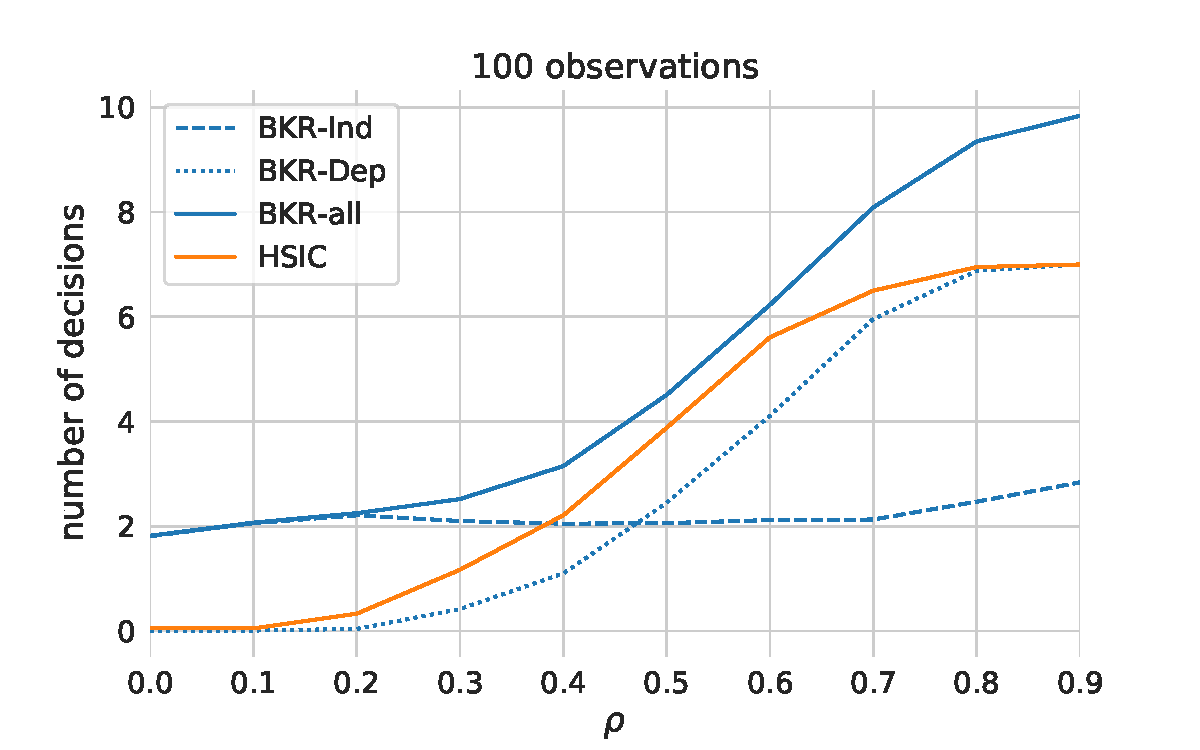
\includegraphics[height=1.9in]{100.pdf}
%     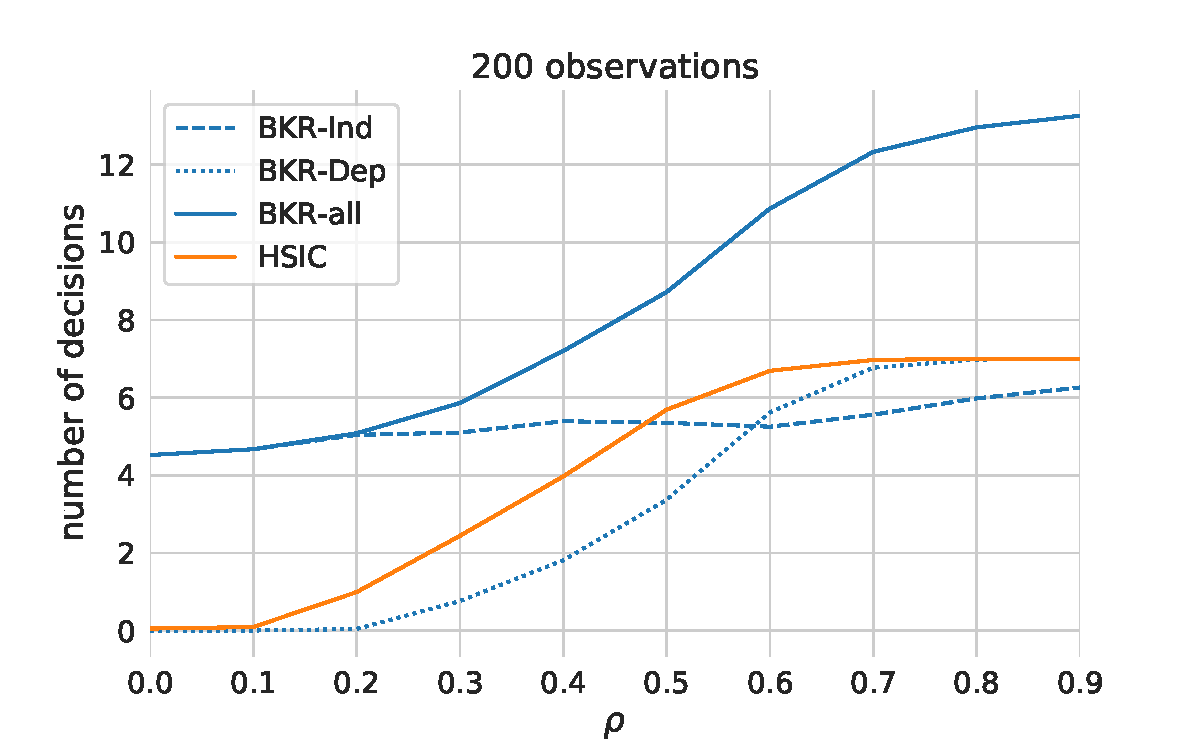
\includegraphics[height=1.9in]{200.pdf}
%   \end{tabular}
%   \caption{Synthetic dataset D1. \textbf{Just an example of figures.}}
%   \label{fig:2}
% \end{figure}


%%------------------------------------------------------------------------------
\section{Other Information}
\label{sec:other}
%%------------------------------------------------------------------------------
\subsection{Data management}
% Responsible data management is part of good research. To promote effective and efficient data management, data sharing and data reuse, we expect researchers to carefully manage data. Research data are the evidence that underpin the answer to research questions, and can be used to validate findings. Data can be quantitative information or qualitative statements collected by researchers in the course of their work by experimentation, observation, modelling, interview or other methods, or information derived from existing evidence.

% We understand software as included in the definition of research data. Algorithms, scripts and code developed by researchers in the course of their work may be necessary to access and interpret data. In such cases, the data management plan will be expected to address how information about such items will be made available.

% Research results should be stored in such a way that they can be retrieved and reproduced and/or reused in the long term, also by researchers in disciplines and organisations other than those in which the research took place. The operating principle is that all stored data are, in principle, freely accessible and that access is only limited if needed for reasons such as privacy, public security, ethical restrictions, property rights and commercial interests. Any tools or software (algorithms, scripts and code developed by researchers in the course of their work) necessary to access and interpret data should be made available alongside the data.

\paragraph*{Will this project involve re-using existing research data?} There are many open-source datasets containing millions of images. These are also widely used in reports to compare various approaches. I will also use these datasets. During development, I am mainly planning on using the Pascal VOC \cite{hoiem2009pascal} datasets. However, in the final report I would like to report on more datasets if the time and compute allows for it.

I would like to also publicly provide any code required to rerun the experiments reported on in the paper, however as this research will be done in collaboration with a company it might not be possible to share all code. All code that can be made public, will be shared posted on GitHub in a public archived repository.

\paragraph*{Will data be collected or generated that are suitable for reuse?} Depending on if the model will be trained using company resources (data and/or compute), the model weights can be reused. If possible I would like to make the weights used for reporting the metrics on Pascal VOC publicly available such that the experiments can easily be repeated by third parties.

\paragraph*{Possible data sharing restrictions} As this project is in collaboration with a company, if company IP is used for (parts of) the research it might not be possible to publicize those parts of the code. However, as this is a research project and does not (necessarily) involve running the code on production units. It is likely that a large part of the code can be made public.


%%------------------------------------------------------------------------------
\subsection{Motivation for choice of research group / supervisor / company}

% This subsection can be used to explain why you have chosen this project with respect to supervisor, group and company. It is used to explain your view on the alignment of topic and the project team.
I chose for this project due to my interest and prior work experience with Object Detection. I have a preference of doing my thesis at a company as I feel like that I would have a more tangible end-goal versus a purely research based project. Furthermore, the robotic background of Avular interests me as I hope to be able to see the results of my work in the real world, applied on physical products.


% Note that the importance of each section and subsection and their respective content and size may vary from proposal to proposal. So you are expected to balance the content and length of each part accordingly. Typically, Section~\ref{sec:other} is considerably smaller than the other sections. Often Sections~\ref{sec:goals}, \ref{sec:approach}, and~\ref{sec:evidence} are the largest sections.



\bibliographystyle{abbrv}
\printbibliography
% \bibliography{references}

\begin{comment}
\appendix
\section{Appendix}

You may provide any type of material as appendix to your project proposal. Typical appendices include additional details about the methodology, further pilot studies for illustration and demonstration of feasibility, images and results that were created, pointers to code (or pseudo-code itself), pointers to data, etc. There is no limit in the length of the appendices. For example, this appendix contain Table~\ref{table:somethinginside}, which has information that are not relevant but shows how to use a table here.

\begin{table}[ht]
  \caption{Some results of something. It is recommend not to try to understand it.\label{table:somethinginside}}
  \begin{center}
    \begin{tabular}{cccc|cc|cc}
              &                &           &       & \multicolumn{2}{c|}{Median} & \multicolumn{2}{c}{Maximum}                       \\
      Problem & Description    & Max Value & Nodes & Memory                      & Time(s)                     & Memory    & Time(s) \\
      \hline
      MINAP   & naive Bayes w/ & $10^{6}$  & 50    & $59$                        & $0.06$                      & $84$      & $0.08$  \\
              & random params  &           & 100   & $125$                       & $0.198$                     & $200$     & $0.285$ \\
              &                &           & 200   & $396$                       & $1.328$                     & $1238$    & $1.893$ \\
              &                &           & 300   & $1103$                      & $2.793$                     & $20863$   & $9.893$ \\
      MAP     & naive Bayes w/ & $10^{6}$  & 50    & $5$                         & $0.01$                      & $7$       & $0.015$ \\
              & random params  &           & 100   & $5$                         & $0.017$                     & $6$       & $0.023$ \\
              &                &           & 200   & $5$                         & $0.04$                      & $7$       & $0.047$ \\
              &                &           & 300   & $5$                         & $0.043$                     & $7$       & $0.049$ \\
      MINAP   & partition      & $10^{4}$  & 10    & $512$                       & $0.034$                     & $512$     & $0.039$ \\
              & problem        &           & 20    & $91857$                     & $11.553$                    & $100842$  & $17.42$ \\
              &                &           & 30    & $236979$                    & $77.09$                     & $264638$  & $82.81$ \\
              &                & $10^{5}$  & 10    & $512$                       & $0.036$                     & $512$     & $0.045$ \\
              &                &           & 20    & $347065$                    & $27.599$                    & $372670$  & $31.10$ \\
              &                &           & 30    & $2046264$                   & $532.318$                   & $2237859$ & $586.4$ \\
              &                & $10^{6}$  & 10    & $512$                       & $0.035$                     & $512$     & $0.038$ \\
              &                &           & 20    & $501347$                    & $34.672$                    & $510413$  & $38.13$ \\
              &                &           & 30    & $>10$Mln                    & $>600$                      & $>10$Mln  & $>600$  \\
      MINAP   & random struct. & $10^{6}$  & 50    & $57$                        & $0.046$                     & $101$     & $0.073$ \\
              & and parameters &           & 100   & $143$                       & $0.21$                      & $197$     & $0.326$ \\
              &                &           & 200   & $417$                       & $1.288$                     & $713$     & $1.761$ \\
              &                &           & 300   & $1129$                      & $2.509$                     & $10403$   & $14.53$ \\
      MAP     & random struct. & $10^{6}$  & 50    & $5$                         & $0.009$                     & $7$       & $0.014$ \\
              & and parameters &           & 100   & $5$                         & $0.018$                     & $6$       & $0.023$ \\
              &                &           & 200   & $5$                         & $0.042$                     & $7$       & $0.047$ \\
              &                &           & 300   & $6$                         & $0.049$                     & $7$       & $0.061$ \\
      \hline
    \end{tabular}
  \end{center}
\end{table}

\lipsum[1-4]
\end{comment}

\end{document}

